\documentclass{standalone}
\usepackage{tikz}
\usepackage{ctex,siunitx}
\usepackage{tkz-euclide}
\usepackage{amsmath}
\usetikzlibrary{patterns, calc}
\usetikzlibrary {decorations.pathmorphing, decorations.pathreplacing, decorations.shapes,}
\begin{document}
\small
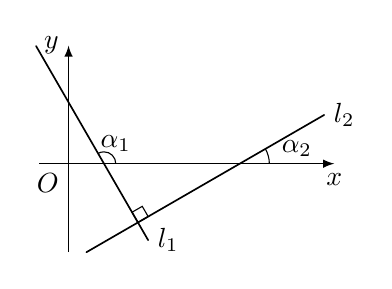
\begin{tikzpicture}[>=latex,scale=0.75]
  \begin{scope}
    \draw[thin,->](-0.5,0)--(4.5,0)node[below]{$x$};
    \draw[thin,->](0,-1.5)--(0,2.0)node[left]{$y$};
    \tkzDefPoints{0.6/0/A,2.9/0/B,4/0/E,0/0/O}
    \tkzDefShiftPoint[B](30:1.5){C}
    \tkzDefPointBy[projection=onto B--C](A)\tkzGetPoint{D}
    \tkzDefShiftPoint[D](120:2.0){D'}
    \tkzDrawLine[semithick,add = 2.0 and 0.1](B,C)
    \tkzLabelLine[pos=1.1,right](B,C){$l_2$}
    \tkzDrawLine[semithick,add = 2.0 and 0.3](A,D)
    \tkzLabelLine[pos=1.3,right](A,D){$l_1$}
    \tkzMarkAngle[size=0.5](E,B,C)
    \tkzLabelAngle[pos=1.0](E,B,C){$\alpha_2$}
    \tkzMarkAngle[size=0.2](E,A,D')
    \tkzLabelAngle[pos=0.4](E,A,D'){$\alpha_1$}
    \tkzMarkRightAngle[size=0.2](A,D,B)
    \tkzLabelPoints[below left](O)
    % \tkzLabelPoints(A,B,E,D)
  \end{scope}
\end{tikzpicture}
\end{document}